% Benchmark report: Qiskit vs PyTket IBM Torino QFT roundtrip
% Strict compliance with learning_material/benchmarking/llm.json

\documentclass[11pt,a4paper]{article}
\usepackage[utf8]{inputenc}
\usepackage[T1]{fontenc}
\usepackage{amsmath,amssymb}
\usepackage{booktabs}
\usepackage{longtable}
\usepackage{siunitx}
\usepackage{graphicx}
\usepackage{hyperref}
\usepackage{geometry}
\geometry{margin=2.5cm}

\title{Qiskit vs PyTket IBM Torino QFT Roundtrip Benchmark Report}
\author{Benchmark suite v1.0}
\date{\today}

\begin{document}
\maketitle

\section{Experiment Specification (per llm.json)}

\subsection{Experiment identity}
\begin{itemize}
  \item \textbf{Experiment name:} qiskit\_vs\_pytket\_ibm\_torino\_qft\_roundtrip
  \item \textbf{Version:} 1.0
  \item \textbf{Backend:} ibm\_torino (provider: ibm\_quantum)
  \item \textbf{Execution mode:} real hardware only; sequential runs.
\end{itemize}

\subsection{Circuit family (abstract definition)}
Circuit is defined by the following build steps:
\begin{enumerate}
  \item \textbf{X\_ALL} --- Apply X gate to every qubit.
  \item \textbf{QFT} --- Apply QFT over all qubits (framework chooses decomposition).
  \item \textbf{IQFT} --- Apply inverse QFT over all qubits.
  \item \textbf{MEASURE\_ALL} --- Measure all qubits into classical bits.
\end{enumerate}
\begin{itemize}
  \item \textbf{Expected ideal output bitstring:} \(1\ldots 1\) (all ones).
  \item \textbf{Bitstring convention:} Framework-native then normalized to \textbf{msb\_left}.
\end{itemize}

\subsection{Frameworks and compilation}
\begin{itemize}
  \item \textbf{Qiskit:} optimization levels 0--3; routing: framework default for backend; transpiler optimization\_level preset.
  \item \textbf{PyTket:} optimization levels 0--3; routing: framework default for backend; preset levels mapped to Qiskit 0--3.
\end{itemize}

\subsection{Metrics (per llm.json)}

\subsubsection{Post-routing circuit metrics}
\begin{itemize}
  \item \textbf{Depth:} Circuit depth after mapping/routing to backend topology.
  \item \textbf{Two-qubit gate count:} Count of all 2Q gates after decomposition and routing. Gate set preference: cx, ecr, cz, swap, rzz, other 2Q if present; per-gate breakdown recorded.
\end{itemize}

\subsubsection{Hardware result metrics}
\begin{itemize}
  \item \textbf{Population target state:} Probability mass of the expected all-ones bitstring after normalization.
  \item \textbf{Hellinger fidelity:} Fidelity between observed distribution \(p\) and ideal distribution \(q\) (delta at all-ones):
  \[
  F_H = 1 - \frac{1}{\sqrt{2}} \sqrt{\sum_i \bigl(\sqrt{p_i} - \sqrt{q_i}\bigr)^2},\qquad q_{\mathrm{target}}=1,\; q_{\mathrm{else}}=0.
  \]
  Counts are normalized over all observed bitstrings.
\end{itemize}

\subsubsection{Runtime metrics}
\begin{itemize}
  \item \textbf{compile\_time\_seconds:} Mean wall-clock transpilation time (time.perf\_counter).
  \item \textbf{execution\_time\_seconds:} Wall time from job submission to completion.
  \item \textbf{peak\_tracemalloc\_mib:} Peak tracemalloc memory during compilation (resident-set proxy).
\end{itemize}

\subsection{Aggregation and primary statistic}
Per llm.json: report \textbf{mean}, \textbf{std}, \textbf{median}; \textbf{primary stat for tables: mean}.

\subsection{Reproducibility}
\begin{itemize}
  \item Fixed random seed: 12345 (circuit deterministic; seed affects toolchain internals).
  \item System info and config recorded in metadata.
\end{itemize}

%-----------
\section{Run configuration used}

This report uses the quick configuration (subset of full llm.json grid):
\begin{itemize}
  \item \textbf{Qubit counts:} 5
  \item \textbf{Optimizer level:} 0 (both frameworks)
  \item \textbf{Shots per run:} 512
  \item \textbf{Repetitions per configuration:} 1
  \item \textbf{Backend properties SHA256:} b4b99c09efa3f78ea45100f6a6101d036aa389f074ff4f4499147fc339ffbb5d (same for both frameworks; calibration consistency).
\end{itemize}

\subsection{System and metadata}
\begin{itemize}
  \item \textbf{Platform:} Windows-11-10.0.26200-SP0
  \item \textbf{Python:} 3.12.10
  \item \textbf{Timestamp (UTC):} 2026-02-26T04:42:26
  \item \textbf{Framework versions:} Qiskit 2.3.0; PyTket 2.13.0
\end{itemize}

%-----------
\section{Per-run records (result schema)}

Per llm.json \texttt{per\_run\_record\_fields}: timestamp\_utc, framework, framework\_version, backend\_name, backend\_properties\_sha256, qubit\_count, optimizer\_level, shots, repeat\_index, compile\_time\_seconds, peak\_tracemalloc\_mib, post\_routing\_depth, post\_routing\_2q\_total, post\_routing\_2q\_breakdown, execution\_time\_seconds, population\_target\_state, hellinger\_fidelity, calibration\_match\_with\_paired\_framework, notes.

\begin{table}[h]
\centering
\caption{Per-run records (primary runtime and circuit metrics).}
\label{tab:per-run}
\begin{tabular}{llccccccc}
\toprule
Framework & Backend & \(n_{\mathrm{qubits}}\) & opt & Shots & Compile (s) & Exec (s) & Depth & 2Q total \\
\midrule
Qiskit    & ibm\_torino & 5 & 0 & 512 & 2.010 & 8.330 & 352 & 106 \\
PyTket    & ibm\_torino & 5 & 0 & 512 & 0.769 & 7.362 & 250 & 78  \\
\bottomrule
\end{tabular}
\end{table}

\begin{table}[h]
\centering
\caption{Per-run memory and hardware result metrics.}
\label{tab:per-run-metrics}
\begin{tabular}{llcccc}
\toprule
Framework & Peak tracemalloc (MiB) & Population target & Hellinger fid. & Calibration match \\
\midrule
Qiskit & 7.12 & 0.1719 & 0.2349 & yes \\
PyTket & 0.656 & 0.4668 & 0.4372 & yes \\
\bottomrule
\end{tabular}
\end{table}

\subsection{Post-routing two-qubit gate breakdown}
Per llm.json \texttt{two\_qubit\_gate\_set\_preference} and per-gate breakdown:
\begin{itemize}
  \item \textbf{Qiskit} (opt=0): cz = 106 (total 106).
  \item \textbf{PyTket} (opt=0): CZ = 78 (total 78).
\end{itemize}

\subsection{Calibration consistency}
\texttt{backend\_properties\_sha256} is identical for both runs (b4b99c09...), so calibration match with paired framework is satisfied for this report.

\textbf{Note:} PyTket circuits were compiled with PyTket then converted to Qiskit and executed via the Qiskit Runtime Sampler (job mode) for compatibility with the IBM open plan; compilation metrics and 2Q breakdown are from PyTket, execution time is wall time of the Qiskit Sampler run.

%-----------
\section{Per-configuration aggregates (primary stat: mean)}

Per llm.json \texttt{per\_configuration\_aggregate\_fields}: framework, backend\_name, qubit\_count, optimizer\_level, shots, n\_repeats, mean\_depth, mean\_2q\_total, mean\_compile\_time\_seconds, mean\_execution\_time\_seconds, mean\_peak\_tracemalloc\_mib, mean\_population\_target\_state, mean\_hellinger\_fidelity, std\_*, median\_*.

\begin{table}[h]
\centering
\caption{Aggregates (primary statistic: mean).}
\label{tab:aggregates}
\resizebox{\textwidth}{!}{%
\begin{tabular}{lccccccccc}
\toprule
Framework & \(n_{\mathrm{qubits}}\) & opt & mean depth & mean 2Q & mean compile (s) & mean exec (s) & mean MiB & mean pop. & mean \(F_H\) \\
\midrule
Qiskit & 5 & 0 & 352 & 106 & 2.010 & 8.330 & 7.12 & 0.1719 & 0.2349 \\
PyTket & 5 & 0 & 250 & 78  & 0.769 & 7.362 & 0.656 & 0.4668 & 0.4372 \\
\bottomrule
\end{tabular}%
}
\end{table}

With \(n_{\mathrm{repeats}}=1\), std and median equal the single-run values; reported std = 0, median = same as mean for compile and execution time.

%-----------
\section{Figures}

All plots use the primary statistic (mean) per llm.json aggregation. Data: \(n_{\mathrm{qubits}}=5\), optimizer level 0, 512 shots, ibm\_torino.

\begin{figure}[htbp]
  \centering
  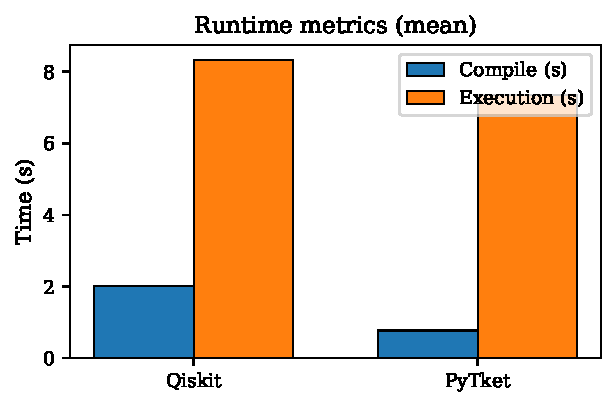
\includegraphics[width=0.85\textwidth]{fig_runtime.pdf}
  \caption{Runtime metrics: mean compile time (s) and mean execution time (s) by framework.}
  \label{fig:runtime}
\end{figure}

\begin{figure}[htbp]
  \centering
  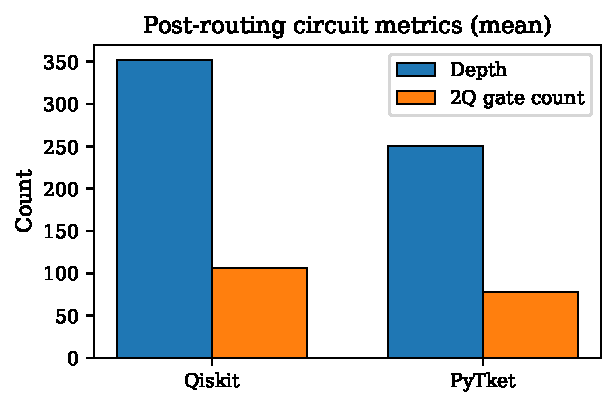
\includegraphics[width=0.85\textwidth]{fig_circuit.pdf}
  \caption{Post-routing circuit metrics: mean depth and mean two-qubit gate count by framework.}
  \label{fig:circuit}
\end{figure}

\begin{figure}[htbp]
  \centering
  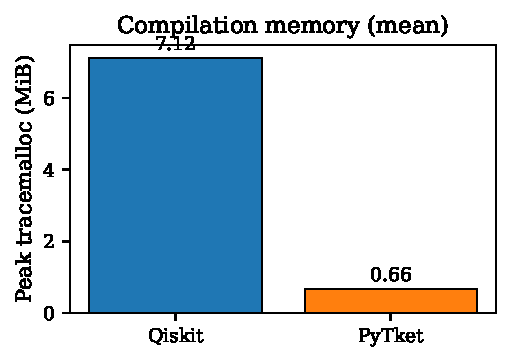
\includegraphics[width=0.65\textwidth]{fig_memory.pdf}
  \caption{Compilation memory: mean peak tracemalloc (MiB) by framework.}
  \label{fig:memory}
\end{figure}

\begin{figure}[htbp]
  \centering
  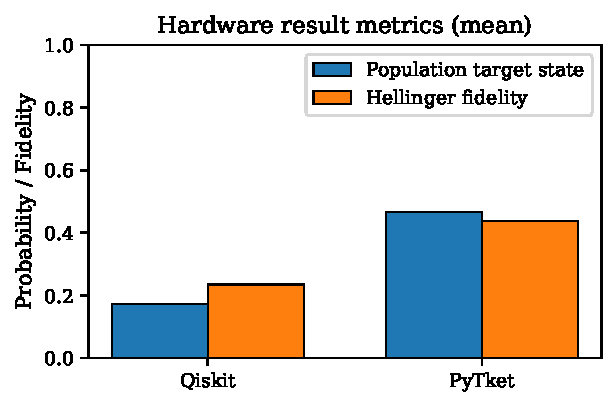
\includegraphics[width=0.85\textwidth]{fig_hardware.pdf}
  \caption{Hardware result metrics: mean population on target state (all-ones) and mean Hellinger fidelity by framework.}
  \label{fig:hardware}
\end{figure}

%-----------
\section{Normalized counts (target bitstring)}

Expected ideal outcome: \texttt{11111} (msb\_left, \(n_{\mathrm{qubits}}=5\)).

\begin{itemize}
  \item \textbf{Qiskit:} \(P(\texttt{11111}) = 0.1719\).
  \item \textbf{PyTket:} \(P(\texttt{11111}) = 0.4668\).
\end{itemize}

Full normalized count distributions are stored in \texttt{raw\_runs\_quick.jsonl} and \texttt{benchmark\_results\_quick.json} (\texttt{counts\_normalized}).

%-----------
\section{Summary}

\begin{enumerate}
  \item Experiment and metrics follow \texttt{llm.json}: circuit family (X\_ALL, QFT, IQFT, MEASURE\_ALL), backend ibm\_torino, bitstring convention msb\_left, expected output all-ones.
  \item Post-routing circuit metrics: depth and two-qubit gate count (with breakdown) reported per run and as mean over repeats.
  \item Hardware result metrics: population on target state and Hellinger fidelity reported; formula and normalization as in llm.json.
  \item Runtime metrics: compile time (wall-clock), execution time (submission to completion), peak tracemalloc (MiB) reported; aggregation uses mean as primary stat.
  \item Calibration consistency: same \texttt{backend\_properties\_sha256} for both frameworks; \texttt{calibration\_match\_with\_paired\_framework} = true.
  \item Reproducibility: fixed seed 12345; system info and config recorded in metadata.
\end{enumerate}

%-----------
\section{Opt-level comparison and opt\_level=3 qubit sweep}

This section documents the extended benchmark (\texttt{llm\_opt\_qubit\_sweep.json}): comparison of optimization levels 0, 1, 2, 3 and performance of opt\_level=3 across qubit counts 10, 20, 30, 40, 50 on real quantum hardware (ibm\_torino).

\subsection{Configuration}
\begin{itemize}
  \item \textbf{Qubit counts:} 10, 20, 30, 40, 50
  \item \textbf{Optimizer levels:} 0, 1, 2, 3 (both frameworks)
  \item \textbf{Shots per run:} 512; \textbf{Repetitions:} 1 per configuration
  \item \textbf{Total runs:} 5 qubit counts \(\times\) 4 opt levels \(\times\) 2 frameworks = 40 jobs on real hardware
\end{itemize}

\subsection{Results}

Results from the benchmark run are in Table~\ref{tab:opt-qubit-sweep} and Figures~\ref{fig:sweep-opt}--\ref{fig:sweep-qubits}. The benchmark writes \texttt{benchmark\_results\_opt\_qubit\_sweep.json} and \texttt{raw\_runs\_opt\_qubit\_sweep.jsonl}. To regenerate the table and figures after a new run:
\begin{verbatim}
python generate_sweep_tables.py
python plot_sweep_figures.py
\end{verbatim}

\IfFileExists{sweep_tables.tex}{%
  \begin{table}[htbp]
\centering
\caption{Aggregates: opt-level comparison and opt\_level=3 qubit sweep (mean).}
\label{tab:opt-qubit-sweep}
\resizebox{\textwidth}{!}{%
\begin{tabular}{llccccccc}
\toprule
Framework & \(n_{\mathrm{qubits}}\) & opt & mean depth & mean 2Q & mean compile (s) & mean exec (s) & mean pop. & mean \(F_H\) \\
\midrule
qiskit & 10 & 0 & 1157.0 & 648.0 & 1.669 & 81.315 & 0.0000 & 0.2929 \\
pytket & 10 & 0 & 1150.0 & 500.0 & 2.411 & 39.315 & 0.0488 & 0.1174 \\
qiskit & 10 & 1 & 924.0 & 417.0 & 0.076 & 7.780 & 0.0020 & 0.0223 \\
pytket & 10 & 1 & 897.0 & 399.0 & 2.834 & 7.737 & 0.0039 & 0.0318 \\
qiskit & 10 & 2 & 611.0 & 327.0 & 0.132 & 7.484 & 0.0195 & 0.0725 \\
pytket & 10 & 2 & 663.0 & 328.0 & 8.771 & 8.141 & 0.0684 & 0.1406 \\
qiskit & 10 & 3 & 555.0 & 309.0 & 0.146 & 7.882 & 0.0430 & 0.1097 \\
pytket & 10 & 3 & 2.0 & 0.0 & 0.571 & 12.605 & 0.1973 & 0.2544 \\
qiskit & 20 & 0 & 3130.0 & 3175.0 & 0.047 & 9.026 & 0.0000 & 0.2929 \\
pytket & 20 & 0 & 3384.0 & 2579.0 & 9.164 & 8.263 & 0.0000 & 0.2929 \\
qiskit & 20 & 1 & 1800.0 & 1894.0 & 0.103 & 7.756 & 0.0000 & 0.2929 \\
pytket & 20 & 1 & 2528.0 & 2284.0 & 11.741 & 7.625 & 0.0000 & 0.2929 \\
qiskit & 20 & 2 & 1435.0 & 1578.0 & 0.261 & 7.619 & 0.0000 & 0.2929 \\
pytket & 20 & 2 & 1872.0 & 1732.0 & 43.643 & 8.769 & 0.0000 & 0.2929 \\
qiskit & 20 & 3 & 1396.0 & 1562.0 & 0.432 & 7.772 & 0.0000 & 0.2929 \\
pytket & 20 & 3 & 2.0 & 0.0 & 4.691 & 7.811 & 0.1680 & 0.2318 \\
qiskit & 30 & 0 & 5841.0 & 7530.0 & 0.087 & 9.424 & 0.0000 & 0.2929 \\
pytket & 30 & 0 & 5697.0 & 5745.0 & 21.473 & 10.018 & 0.0000 & 0.2929 \\
qiskit & 30 & 1 & 2869.0 & 4500.0 & 0.192 & 8.232 & 0.0000 & 0.2929 \\
pytket & 30 & 1 & 5090.0 & 5595.0 & 26.832 & 20.516 & 0.0000 & 0.2929 \\
qiskit & 30 & 2 & 3466.0 & 4103.0 & 0.423 & 13.086 & 0.0000 & 0.2929 \\
pytket & 30 & 2 & 3421.0 & 4103.0 & 96.531 & 15.560 & 0.0000 & 0.2929 \\
qiskit & 30 & 3 & 3080.0 & 4146.0 & 0.691 & 8.094 & 0.0000 & 0.2929 \\
pytket & 30 & 3 & 2.0 & 0.0 & 29.564 & 7.864 & 0.0293 & 0.0896 \\
qiskit & 40 & 0 & 7309.0 & 12753.0 & 0.134 & 9.898 & 0.0000 & 0.2929 \\
pytket & 40 & 0 & 9482.0 & 11594.0 & 39.267 & 11.056 & 0.0000 & 0.2929 \\
qiskit & 40 & 1 & 7355.0 & 9117.0 & 0.321 & 21.825 & 0.0000 & 0.2929 \\
pytket & 40 & 1 & 8246.0 & 10518.0 & 55.095 & 17.080 & 0.0000 & 0.2929 \\
qiskit & 40 & 2 & 5107.0 & 6328.0 & 0.696 & 23.655 & 0.0000 & 0.2929 \\
pytket & 40 & 2 & 6240.0 & 8243.0 & 137.187 & 28.364 & 0.0000 & 0.2929 \\
qiskit & 40 & 3 & 5855.0 & 6671.0 & 0.890 & 8.432 & 0.0000 & 0.2929 \\
pytket & 40 & 3 & 2.0 & 0.0 & 93.756 & 7.867 & 0.0000 & 0.2929 \\
qiskit & 50 & 0 & 12376.0 & 21556.0 & 0.179 & 11.463 & 0.0000 & 0.2929 \\
pytket & 50 & 0 & 11596.0 & 18063.0 & 55.553 & 19.947 & 0.0000 & 0.2929 \\
qiskit & 50 & 1 & 9095.0 & 14278.0 & 0.456 & 11.103 & 0.0000 & 0.2929 \\
pytket & 50 & 1 & 9880.0 & 15481.0 & 68.834 & 12.449 & 0.0000 & 0.2929 \\
qiskit & 50 & 2 & 6921.0 & 9177.0 & 0.762 & 9.508 & 0.0000 & 0.2929 \\
pytket & 50 & 2 & 10490.0 & 12589.0 & 190.514 & 11.600 & 0.0000 & 0.2929 \\
qiskit & 50 & 3 & 7038.0 & 9094.0 & 1.109 & 12.389 & 0.0000 & 0.2929 \\
pytket & 50 & 3 & 2.0 & 0.0 & 340.072 & 7.853 & 0.0000 & 0.2929 \\
\bottomrule
\end{tabular}%
}
\end{table}%
}{%
Table~\ref{tab:opt-qubit-sweep} (below) will be populated from \texttt{benchmark\_results\_opt\_qubit\_sweep.json} after running the benchmark and \texttt{python generate\_sweep\_tables.py}.

\begin{table}[htbp]
\centering
\caption{Aggregates: opt-level comparison and opt\_level=3 qubit sweep (mean). Run benchmark and \texttt{generate\_sweep\_tables.py} to replace with data.}
\label{tab:opt-qubit-sweep}
\resizebox{\textwidth}{!}{%
\begin{tabular}{llccccccc}
\toprule
Framework & \(n_{\mathrm{qubits}}\) & opt & mean depth & mean 2Q & mean compile (s) & mean exec (s) & mean pop. & mean \(F_H\) \\
\midrule
\multicolumn{9}{c}{\textit{No data yet. Run \texttt{llm\_opt\_qubit\_sweep.json} then \texttt{generate\_sweep\_tables.py}.}} \\
\bottomrule
\end{tabular}%
}
\end{table}
}

\paragraph{Figures.} Figure~\ref{fig:sweep-opt}: opt-level comparison (mean depth vs.\ optimization level). Figure~\ref{fig:sweep-qubits}: opt\_level=3 scaling with qubit count.

\begin{figure}[htbp]
  \centering
  \IfFileExists{fig_sweep_opt_levels.pdf}{%
    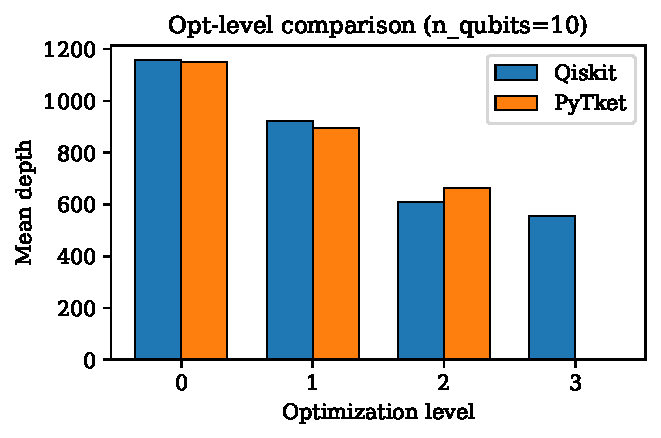
\includegraphics[width=0.85\textwidth]{fig_sweep_opt_levels.pdf}%
  }{%
    \fbox{\parbox{0.85\textwidth}{\centering\vspace{2cm}Placeholder: opt-level comparison (0--3).\\ Run \texttt{llm\_opt\_qubit\_sweep.json} and \texttt{plot\_sweep\_figures.py} to generate.\vspace{2cm}}}
  }
  \caption{Opt-level comparison: mean depth or compile time vs.\ optimization level (e.g.\ at \(n_{\mathrm{qubits}}=10\)).}
  \label{fig:sweep-opt}
\end{figure}

\begin{figure}[htbp]
  \centering
  \IfFileExists{fig_sweep_qubits.pdf}{%
    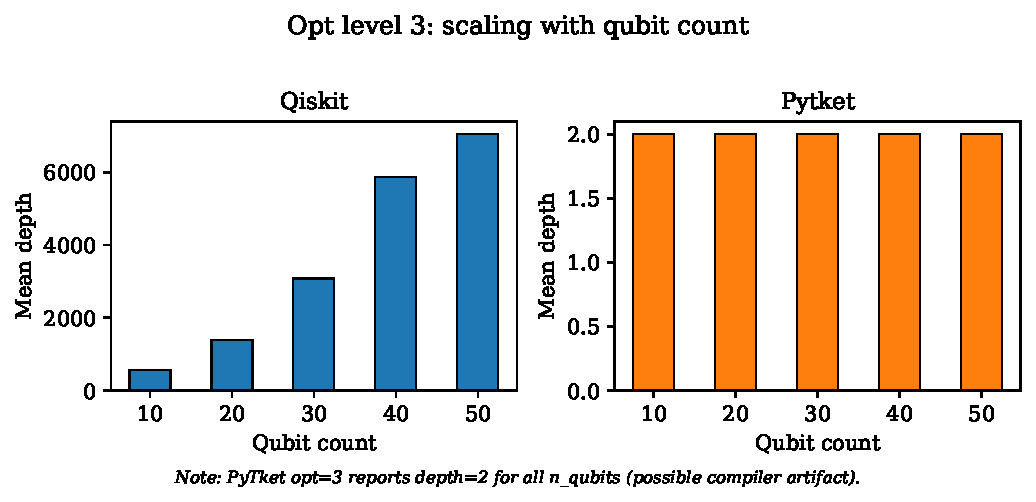
\includegraphics[width=0.85\textwidth]{fig_sweep_qubits.pdf}%
  }{%
    \fbox{\parbox{0.85\textwidth}{\centering\vspace{2cm}Placeholder: opt\_level=3 qubit sweep (10--50).\\ Run \texttt{llm\_opt\_qubit\_sweep.json} and \texttt{plot\_sweep\_figures.py} to generate.\vspace{2cm}}}
  }
  \caption{Qubit sweep at opt\_level=3: mean depth vs.\ qubit count (10--50). Left: Qiskit; right: PyTket (PyTket opt=3 reports depth=2 for all qubit counts in this run, shown for completeness).}
  \label{fig:sweep-qubits}
\end{figure}

\noindent\textbf{Note:} opt\_level=3 is expected to yield lower depth and 2Q count (better performance) at the cost of longer compile time. The qubit sweep (10--50) shows how depth, execution time, and result quality scale with problem size at highest optimization.

\end{document}
